\documentclass[convert={density=300,size=1080x800,outext=.png}]{standalone}
\usepackage{tkz-graph}
\usetikzlibrary{arrows,positioning,shapes,shapes.multipart,patterns,mindmap,shadows}
\usepackage{xcolor}
\usepackage{helvet}
\renewcommand{\familydefault}{\sfdefault}

\begin{document}

\begin{tiny}
    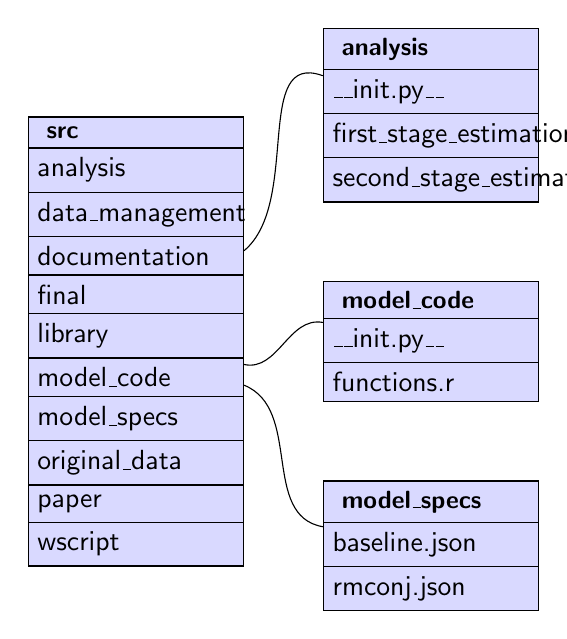
\begin{tikzpicture}[node distance=1cm, auto]
        \node (8) [
            rectangle split,
            rectangle split parts=3,
            rectangle split part fill={
                blue!15,
                blue!15,
                blue!15,
            },
            draw,
            text width=2.5cm
        ]
        {
            \nodepart{one}
                \begin{small}
                    \textbf{model\_code}
                \end{small}
            \nodepart{two}
                \_\_init.py\_\_
            \nodepart{three}
                functions.r
        };

        \node (11) [
            rectangle split,
            rectangle split parts=4,
            rectangle split part fill={
                blue!15,
                blue!15,
                blue!15,
                blue!15,
            },
            draw,
            text width=2.5cm,
            above=of 8
        ]
        {
            \nodepart{one}
                \begin{small}
                    \textbf{analysis}
                \end{small}
            \nodepart{two}
                \_\_init.py\_\_
            \nodepart{three}
                first\_stage\_estimation.r
            \nodepart{four}
                second\_stage\_estimation.r
            \nodepart{five}
                wscript
        };

        \node (222) [
            rectangle split,
            rectangle split parts=3,
            rectangle split part fill={
                blue!15,
                blue!15,
                blue!15,
            },
            draw,
            text width=2.5cm,
            below= of 8
        ]
        {
            \nodepart{one}
                \begin{small}
                    \textbf{model\_specs}
                \end{small}
            \nodepart{two}
                baseline.json
            \nodepart{three}
                rmconj.json
            \nodepart{four}
                geography.json
        };

        \node (3) [
            rectangle split,
            rectangle split parts=11,
            rectangle split part fill={
                blue!15,
                blue!15,
                blue!15,
                blue!15,
                blue!15,
                blue!15,
                blue!15,
                blue!15,
                blue!15,
                blue!15,
                blue!15
            },
            draw,
            text width=2.50cm,
            left=of 8
        ]
        {
            \nodepart{one}
                \begin{small}
                    \textbf{src}
                \end{small}
            \nodepart{two}
                analysis
            \nodepart{three}
                data\_management
            \nodepart{four}
                documentation
            \nodepart{five}
                final
            \nodepart{six}
                library
            \nodepart{seven}
                model\_code
            \nodepart{eight}
                model\_specs
            \nodepart{nine}
                original\_data
            \nodepart{ten}
                paper
            \nodepart{eleven}
                wscript
        };

        \draw[-, out=40, in=160] (3) to (11);
        \draw[-, out=-12, in=170] (3) to (8);
        \draw[-, out=-22, in=170] (3) to (222);
    \end{tikzpicture}
\end{tiny}


\end{document}
